\documentclass{article}
\usepackage{civ}
\newcommand*{\tabbox}[2][t]{%
    \vspace{0pt}\parbox[#1][3.7\baselineskip]{1cm}{\strut#2\strut}}
\title{CIV102: Problem Set \#7}
\author{QiLin Xue \\ \href{mailto:qilin.xue@mail.utoronto.ca}{qilin.xue@mail.utoronto.ca} \\ TA: Michel}
\everymath{\displaystyle}
\usepackage{multirow}
\date{\today}
\usepackage{mathrsfs}
\usetikzlibrary{arrows}
\usetikzlibrary{arrows.meta}
\usepackage{siunitx}
\usepackage{wasysym}
\usetikzlibrary{calc}
\usepackage{xcolor}
\setlength\parindent{0pt}
% \setlength\extrarowheight{10pt}
\renewcommand{\arraystretch}{2}
\usepackage{adjustbox}
\begin{document}
\maketitle
\section{Problem One: Diagrams}
We first solve for the reaction forces at the two supports, which we call $A$ and $B$ respectively from left to right. The net force in the vertical direction is equal to zero, or:
\begin{equation}
    A+B=200+200+60(8)
    \label{eq:}
\end{equation}
Since the system is symmetric about the center vertical axis, we must have $A=B$, which gives us:
\begin{equation}
    A=B=440\si{\kilo\newton}.
    \label{eq:}
\end{equation}
Now, we draw the shear force diagrams:
\begin{center}
    \begin{tikzpicture}
        \draw[thick,->] (0,0) -- (9,0) node[above] {$x(\si{\meter})$};
        \draw[thick,<->] (0,-5) -- (0,5) node[right] {$V(\si{\kilo\newton})$};
        \draw[thick, blue] (0,4.4) -- (3,2.6) -- (3,0.6) -- (5,-0.6) -- (5,-2.6) -- (8,-4.4) -- (8,0);

        \foreach \x in {1,2,...,8}
        {        
          \coordinate (A\x) at ($(0,0)+(\x,0)$) {};
          \draw[ultra thick] ($(A\x)+(0,3pt)$) -- ($(A\x)-(0,3pt)$);
          \node at ($(A\x)+(1ex,-2ex)$) {\x};
        }
        \foreach \y in {440,260,60,-60,-260,-440,0}
        {        
          \coordinate (B\y) at ($(0,0)+(0,\y/100)$) {};
          \draw[ultra thick] ($(B\y)+(3pt,0)$) -- ($(B\y)-(3pt,0)$);
          \node at ($(B\y)+(-4ex,0)$) {\y};
        }

        \draw[dashed] (0,4.4) -- (2,4.4) node[above] {$V_\text{max}$};
        \draw[dashed] (8,-4.4) -- (10,-4.4) node[above] {$V_\text{max}$};

        \end{tikzpicture}
\end{center}
as well as the moment diagram:
\begin{center}
    \begin{tikzpicture}
        \draw[thick,->] (0,0) -- (9,0) node[above] {$x(\si{\meter})$};
        \draw[thick,->] (0,0) -- (0,11) node[right] {$M(\si{\kilo\newton\meter})$};

        \foreach \x in {1,2,...,8}
        {        
          \coordinate (A\x) at ($(0,0)+(\x,0)$) {};
          \draw[ultra thick] ($(A\x)+(0,3pt)$) -- ($(A\x)-(0,3pt)$);
          \node at ($(A\x)+(1ex,-2ex)$) {\x};
        }
        \foreach \y in {0,200,400,...,1000,1050,1080}
        {        
          \coordinate (B\y) at ($(0,0)+(0,\y/100)$) {};
          \draw[ultra thick] ($(B\y)+(3pt,0)$) -- ($(B\y)-(3pt,0)$);
          \node at ($(B\y)+(-4ex,0)$) {\y};
        }
        \draw[blue, thick]  plot[smooth,domain=0:3] (\x, {4.4*\x-0.3*\x*\x});
        \draw[blue, thick] (4,10.8) parabola (3,10.5);
        \draw[blue, thick] (4,10.8) parabola (5,10.5);
        \draw[blue, thick]  plot[smooth,domain=5:8] (\x, {4.4*(\x+6.666)-0.3*(\x+6.666)*(\x+6.666)});

        \draw[dotted] (3,0) -- (3,10.5);
        \draw[dotted] (4,0) -- (4,10.8);
        \draw[dotted] (5,0) -- (5,10.5);
        \draw[dotted] (0,10.5) -- (5,10.5);
        \draw[dotted] (0,10.8) -- (4,10.8);

        \draw (4,10.8) node[above] {$M_\text{max}$}; 
        \end{tikzpicture}
\end{center}
The moment of inertia of the I beam is:
\begin{equation}
    \frac{b_{f}d^{3}}{12}-\frac{\left(b_{f}-b_{w}\right)\left(d-2t_{f}\right)^{3}}{12} = 2843.8 \times 10^6 \si{\milli\meter\tothe{4}}
    \label{eq:}
\end{equation}
and the distance from the neutral axis to both the top and the bottom is:
\begin{equation}
    y = \frac{711}{2} = 355.5\si{\milli\meter}
    \label{eq:}
\end{equation}
so the magnitude of the maximum compressive and tensile stress is:
\begin{equation}
    \sigma = \frac{M_\text{max}y}{I} = 135.0 \si{\mega\pascal}.
    \label{eq:}
\end{equation}
These maximum stresses will occur at the place where the moment is the greatest, which from the diagram is at the middle of the beam. The top shortens and the bottom elongates so the top of the beam will experience compressive stresses while the bottom will experience tensile stresses.
\newpage
\section{Problem 2: Wooden Beam}
We do the same thing, again abusing symmetry. The force from each support will be equal to each other, which we can call $F$. Therefore:
\begin{equation}
    2F = 90(7) \implies F = 315\si{\kilo\newton}
    \label{eq:}
\end{equation}
We can draw a shear force diagram:
\begin{center}
    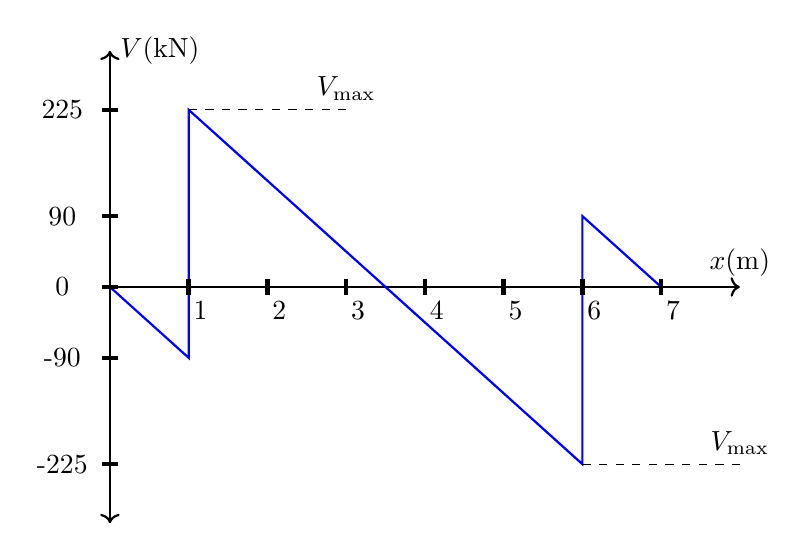
\begin{tikzpicture}
        \draw[thick,->] (0,0) -- (8,0) node[above] {$x(\si{\meter})$};
        \draw[thick,<->] (0,-3) -- (0,3) node[right] {$V(\si{\kilo\newton})$};
        \draw[thick, blue] (0,0) -- (1,-0.9) -- (1,2.25) -- (6,-2.25) -- (6,0.9) -- (7,0);

        \foreach \x in {1,2,...,7}
        {        
          \coordinate (A\x) at ($(0,0)+(\x,0)$) {};
          \draw[ultra thick] ($(A\x)+(0,3pt)$) -- ($(A\x)-(0,3pt)$);
          \node at ($(A\x)+(1ex,-2ex)$) {\x};
        }
        \foreach \y in {0,-90,225,-225,90}
        {        
          \coordinate (B\y) at ($(0,0)+(0,\y/100)$) {};
          \draw[ultra thick] ($(B\y)+(3pt,0)$) -- ($(B\y)-(3pt,0)$);
          \node at ($(B\y)+(-4ex,0)$) {\y};
        }

        \draw[dashed] (1,2.25) -- (3,2.25) node[above] {$V_\text{max}$};
        \draw[dashed] (6,-2.25) -- (8,-2.25) node[above] {$V_\text{max}$};

        \end{tikzpicture}
\end{center}
and a moment diagram:
\begin{center}
    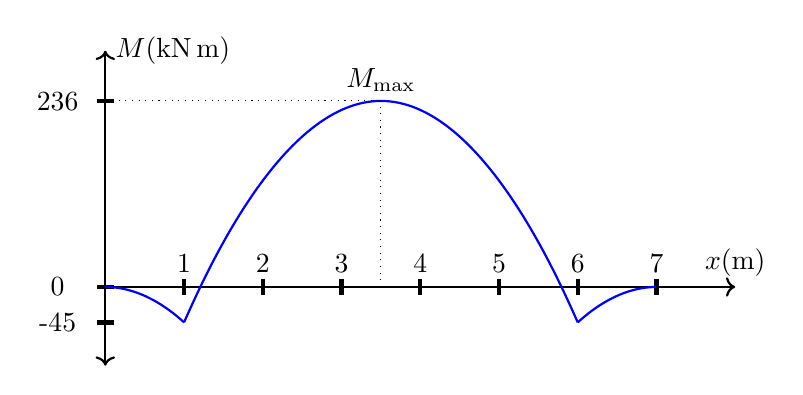
\begin{tikzpicture}
        \draw[thick,->] (0,0) -- (8,0) node[above] {$x(\si{\meter})$};
        \draw[thick,<->] (0,-1) -- (0,3) node[right] {$M(\si{\kilo\newton\meter})$};

        \foreach \x in {1,...,7}
        {        
          \coordinate (A\x) at ($(0,0)+(\x,0)$) {};
          \draw[ultra thick] ($(A\x)+(0,3pt)$) -- ($(A\x)-(0,3pt)$);
          \node at ($(A\x)+(0,2ex)$) {\x};
        }
        \foreach \y in {0,-45,236}
        {        
          \coordinate (B\y) at ($(0,0)+(0,\y/100)$) {};
          \draw[ultra thick] ($(B\y)+(3pt,0)$) -- ($(B\y)-(3pt,0)$);
          \node at ($(B\y)+(-4ex,0)$) {\y};
        }
        % \draw[blue, thick]  plot[smooth,domain=0:3] (\x, {4.4*\x-0.3*\x*\x});

        \draw[blue, thick] (0,0) parabola (1,-0.45);
        \draw[blue, thick] (3.5,2.3625) parabola (1,-0.45);
        \draw[blue, thick] (3.5,2.3625) parabola (6,-0.45);
        \draw[blue, thick] (7,0) parabola (6,-0.45);

        \draw (3.5,2.3625) node[above] {$M_\text{max}$}; 
        \draw [dotted] (0,2.3625) -- (3.5,2.3625);
        \draw [dotted] (3.5,0) -- (3.5,2.3625);
        \end{tikzpicture}
\end{center}
Again, since the top and bottom are equidistant from the neutral line, the maximum tensile and compressive stresses are the same. The moment of inertia of the wooden beam is:
\begin{equation}
    I = \frac{w^4}{12} = 1338.5 \times 10^{6} \si{\milli\meter\tothe{4}}
    \label{eq:}
\end{equation}
such that the tensile and compressive stresses are:
\begin{equation}
    \sigma = \frac{M_\text{max}y}{I} = 31.38 \si{\mega\pascal}.
    \label{eq:}
\end{equation}
Using the ultimate compressive strength of $50\si{\mega\pascal}$, I get:
\begin{equation}
    FOS = 1.593
    \label{eq:}
\end{equation}
and if we wanted the factor of safety against tensile forces, then it is:
\begin{equation}
    FOS_\text{tensile} = \frac{70}{31.38} = 2.23
    \label{eq:}
\end{equation}
\newpage
\section{Problem Three: Truss Bridge}
\textbf{(a)} Refer to the following diagram, with the symmetry axis drawn.
\begin{center}
  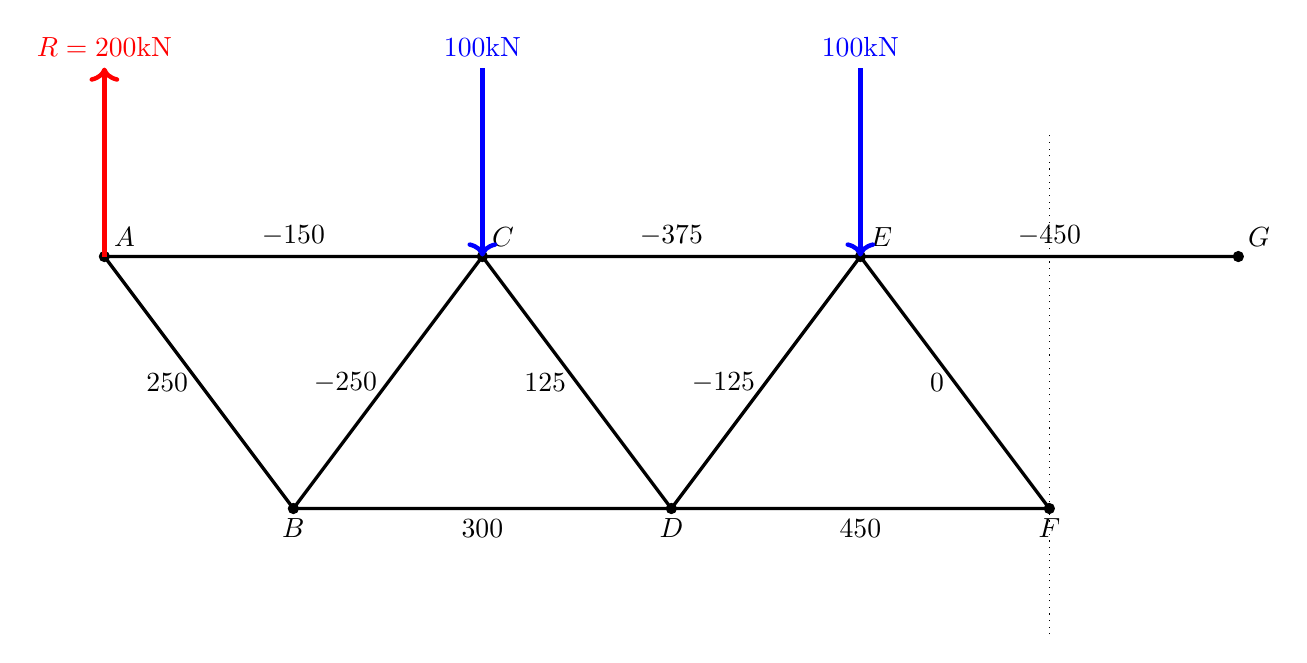
\begin{tikzpicture}[scale=0.8]
    \coordinate (A) at (0,0);
    \coordinate (C) at (6,0);
    \coordinate (E) at (12,0);
    \coordinate (G) at (18,0);

    \coordinate (B) at (3,-4);
    \coordinate (D) at (9,-4);
    \coordinate (F) at (15,-4);
    \draw[dotted] (15,-6) -- (15,2);

    \draw[fill=black] (A) circle (0.08) node[above right] {$A$};
    \draw[fill=black] (C) circle (0.08) node[above right] {$C$};
    \draw[fill=black] (E) circle (0.08) node[above right] {$E$};
    \draw[fill=black] (G) circle (0.08) node[above right] {$G$};
    \draw[fill=black] (B) circle (0.08) node[below] {$B$};
    \draw[fill=black] (D) circle (0.08) node[below] {$D$};
    \draw[fill=black] (F) circle (0.08) node[below] {$F$};

    \draw[very thick] (G)
    -- (E) node[midway,above] {$-450$}
    -- (C) node[midway,above] {$-375$}
    -- (A) node[midway,above] {$-150$}
    -- (B) node[midway,left] {$250$}
    -- (D) node[midway,below] {$300$}
    -- (F) node[midway,below] {$450$}
    -- (E) node[midway,left] {$0$}
    -- (D) node[midway,left] {$-125$}
    -- (C) node[midway,left] {$125$}
    -- (B) node[midway,left] {$-250$};

    \draw[ultra thick, blue, <-] (C) -- ++(0,3) node[above] {$100\si{\kilo\newton}$};
    \draw[ultra thick, blue, <-] (E) -- ++(0,3) node[above] {$100\si{\kilo\newton}$};
    \draw[ultra thick, red, ->] (A) -- ++(0,3) node[above] {$R=200\si{\kilo\newton}$};
  \end{tikzpicture}
\end{center}
The two reaction forces support the entire $400\si{\kilo\newton}$ load, so that each of the reaction forces have a force:
\begin{equation}
  R = 200\si{\kilo\newton}
  \label{eq:}
\end{equation}
and since there are no external horizontal loads and the rightmost support is a roller, none of the supports will exert a horizontal force. Looking at vertical forces, and the vertical component of the force of each beam, we have:
\begin{align*}
  AB_y &= 200\si{\kilo\newton} \\
  BC_y &= -200\si{\kilo\newton} \\ 
  CD_y &= -(100+BC_y) 100\si{\kilo\newton} \\ 
  DE_y &= -100\si{\kilo\newton} \\ 
  EF_y &= 0\si{\kilo\newton}
\end{align*}
We can calculate their actual force by multiplying by $\frac{5}{4}$ and we can determine their horizontal component by multiplying by $\frac{3}{4}$ to get:
\begin{align*}
  AB &= 250\si{\kilo\newton} \\
  BC &= -250\si{\kilo\newton} \\ 
  CD &= 125\si{\kilo\newton} \\ 
  DE &= -125\si{\kilo\newton} \\ 
  EF &= 0\si{\kilo\newton}
\end{align*}
and
\begin{align*}
  AB_x &= 150\si{\kilo\newton} \\
  BC_x &= -150\si{\kilo\newton} \\ 
  CD_x &= 75\si{\kilo\newton} \\ 
  DE_x &= -75\si{\kilo\newton} \\ 
  EF_x &= 0\si{\kilo\newton}
\end{align*}
We can then determine the forces in the horizontal members to be:
\begin{align*}
  AC &= -AB_x = -150\si{\kilo\newton} \\ 
  CE &= AC+BC_x-CD_x = -375\si{\kilo\newton} \\ 
  EG &= CE+DE_x-EF_x = -450\si{\kilo\newton} \\ 
  BD &= AB_x - BC_x = 300\si{\kilo\newton} \\ 
  DF &= BD+CD_x-DE_x = 450\si{\kilo\newton}
\end{align*}
\textbf{(b)} Top chord members are made from HSS 203x203x6.4, which has an area and moment of inertia of:
\begin{align}
  A &= 4900 \si{\milli\meter\squared} \\ 
  I &= 31.3 \times 10^6 \si{\milli\meter\tothe{4}}
  \label{eq:}
\end{align}
The strongest compression force is $EG$, which has both a minimum angle and moment of inertia of:
\begin{align}
  A_\text{min} &= \frac{F}{\sigma} = 1286 \si{\milli\meter\squared} \\ 
  I_\text{min} &= \frac{FL^2}{\pi I} = 8.21 \times 10^6 \si{\milli\meter\tothe{4}}
\end{align}
For a factor of safety of $FOS = 3.81, 3.81$. For the bottom chords, HSS 152x152x4.8 were used, which has an area and moment of inertia of:
\begin{align}
  A &= 2760\si{\milli\meter\squared} \\ 
  I &= 9.93 \times 10^6 \si{\milli\meter\tothe{4}}
\end{align}
The strongest force is $DF$, and there are no forces of compression, so the minimum area needed is:
\begin{equation}
  A_\text{min} = \frac{F}{\sigma} = 1286 \si{\milli\meter\squared}
  \label{eq:}
\end{equation}
for a factor of safety of $FOS=2.15$. Finally for the diagonal chords, they are made of HSS 127x127x8.0, so their area and moment of inertia are:
\begin{align}
  A &= 3620 \si{\milli\meter\squared} \\ 
  I &= 7.05 \times 10^6 \si{\milli\meter\tothe{4}}
\end{align}
The stronger compression force is $BC$, so the minimum area and moment of inertia needed are:
\begin{align}
  A_\text{min} &= \frac{F}{\sigma} = 714 \si{\milli\meter\squared} \\ 
  I_\text{min} &= \frac{FL^2}{\pi I} = 3.17 \times 10^6 \si{\milli\meter\tothe{4}}
\end{align}
so the factors of safety are $FOS=5.07, 2.22$ respectively. We pick the smallest factor of safety, which happens to be $\boxed{FOS=2.22}$.

\textbf{(c)} We use the principle of virtual work, which we can do by drawing another diagram:
\begin{center}
  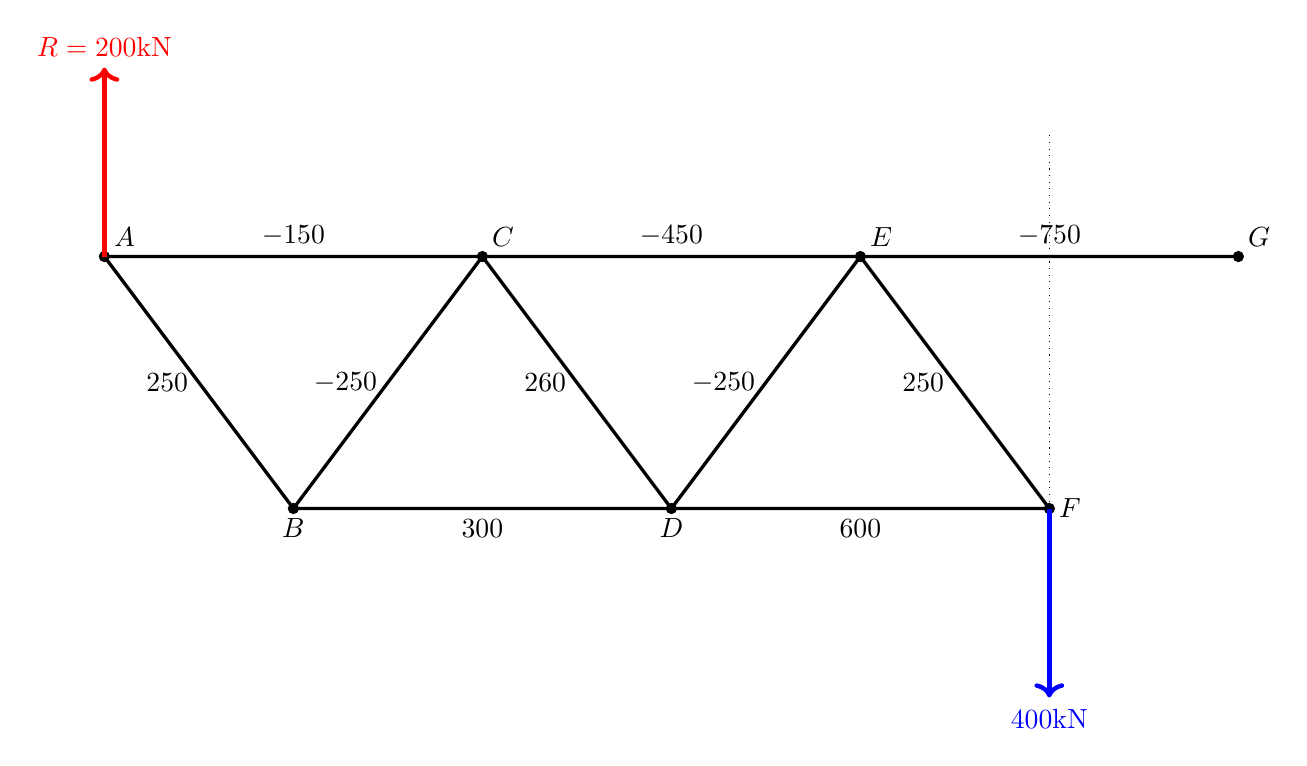
\begin{tikzpicture}[scale=0.8]
    \coordinate (A) at (0,0);
    \coordinate (C) at (6,0);
    \coordinate (E) at (12,0);
    \coordinate (G) at (18,0);

    \coordinate (B) at (3,-4);
    \coordinate (D) at (9,-4);
    \coordinate (F) at (15,-4);
    \draw[dotted] (15,-6) -- (15,2);

    \draw[fill=black] (A) circle (0.08) node[above right] {$A$};
    \draw[fill=black] (C) circle (0.08) node[above right] {$C$};
    \draw[fill=black] (E) circle (0.08) node[above right] {$E$};
    \draw[fill=black] (G) circle (0.08) node[above right] {$G$};
    \draw[fill=black] (B) circle (0.08) node[below] {$B$};
    \draw[fill=black] (D) circle (0.08) node[below] {$D$};
    \draw[fill=black] (F) circle (0.08) node[right] {$F$};

    \draw[very thick] (G)
    -- (E) node[midway,above] {$-750$}
    -- (C) node[midway,above] {$-450$}
    -- (A) node[midway,above] {$-150$}
    -- (B) node[midway,left] {$250$}
    -- (D) node[midway,below] {$300$}
    -- (F) node[midway,below] {$600$}
    -- (E) node[midway,left] {$250$}
    -- (D) node[midway,left] {$-250$}
    -- (C) node[midway,left] {$260$}
    -- (B) node[midway,left] {$-250$};

    \draw[ultra thick, blue, ->] (F) -- ++(0,-3) node[below] {$400\si{\kilo\newton}$};
    \draw[ultra thick, red, ->] (A) -- ++(0,3) node[above] {$R=200\si{\kilo\newton}$};
  \end{tikzpicture}
\end{center}
Again, we can look at the vertical components of the forces, which for all diagonal members happen to be $200\si{\kilo\newton}$, but alternating from tension to compression. The magnitude of their horizontal and actual components are $150\si{\kilo\newton}$ and $250\si{\kilo\newton}$, respectively. Then for the horizontal chords
\begin{align}
  AC &= -150 \si{\kilo\newton} \\ 
  CE &= 450 \si{\kilo\newton} \\ 
  EG &= -750 \si{\kilo\newton}
\end{align}
and for the bottom chords:
\begin{align}
  BD &= 300 \si{\kilo\newton} \\ 
  DF &= 600 \si{\kilo\newton}
\end{align}
We can draw a table:
\begin{center}
  \begin{tabular}{|c|c|c|c|c|c|}
    \hline
    Member & $P$ ($\si{\kilo\newton}$) & $P^*$ ($\si{\kilo\newton}$) & HSS Area ($\si{\milli\meter\squared}$) & Length ($\si{\meter}$) & $\frac{PP^*\ell}{EA} ($\si{\joule}$)$ \\ \hline
    $BD$ &         300          &          300            & \multirow{2}{*}{2760} & \multirow{4}{*}{6} &          978.26             \\ \cline{1-3} \cline{6-6} 
    $DF$ &         450          &          600            &                       &                    &          2934.8            \\ \cline{1-4} \cline{6-6} 
    $AC$ &         150          &          150            & \multirow{3}{*}{4900} &                    &          137.76             \\ \cline{1-3} \cline{6-6} 
    $CE$ &         375          &          450            &                       &                    &          1033.16            \\ \cline{1-3} \cline{5-6} 
    $EG$ &         450          &          750            &                       &         3          &          1033.16            \\ \hline
    $AB$ & \multirow{2}{*}{250} & \multirow{5}{*}{250}    & \multirow{5}{*}{3620} & \multirow{5}{*}{5} &          431.63             \\ \cline{1-1} \cline{6-6} 
    $BC$ &                      &                         &                       &                    &          431.63             \\ \cline{1-2} \cline{6-6} 
    $CD$ & \multirow{2}{*}{125} &                         &                       &                    &          215.81             \\ \cline{1-1} \cline{6-6} 
    $DE$ &                      &                         &                       &                    &          215.81             \\ \cline{1-2} \cline{6-6} 
    $EF$ &           0          &                         &                       &                    &          0                  \\ \hline
    \end{tabular}
\end{center}
When the last column is added up, it gives us:
\begin{equation}
  2\sum \frac{P_iP_i^* \ell_i}{EA} = 14824.04 \si{\joule}
  \label{eq:}
\end{equation}
The principle of virtual work tells us that:
\begin{equation}
  F\Delta L =  \sum \frac{P_iP_i^* \ell_i}{EA}
  \label{eq:}
\end{equation}
Since $F=400 \si{\kilo\newton}$, we have:
\begin{equation}
  \Delta L = \frac{14724.04}{400} = 37.06 \si{\milli\meter}
  \label{eq:}
\end{equation}
so the maximum deformation at point $F$ is $\boxed{\Delta_F = 37.1\si{\milli\meter}}$.
Since the bridge has a distributed load, the natural frequency of oscillations is given by:
\begin{equation}
  f_n = \frac{17.75}{\sqrt{\Delta_F}} = \boxed{2.92\si{\hertz}}
  \label{eq:}
\end{equation}
\textbf{(d)} The dynamic amplification factor is given by:
\begin{equation}
  DAF = \frac{1}{\sqrt{\left(1-\left(\frac{f}{f_n}\right)^2\right)^2+\left(\frac{2\beta f}{f_n}\right)^2}}
  \label{eq:}
\end{equation}
Letting $\beta=0.03$, $f_n=2.917\si{\hertz}$, and $f=2.75\si{\hertz}$, we get a value of $DAF=8.014$. The equivalent static load is then:
\begin{equation}
  w_\text{eq} = w_\text{stationary} + (DAF)w_o = 100 + 8.014(25)=300.35\si{\kilo\newton}
  \label{eq:}
\end{equation}
which is around a factor of $\alpha = \frac{w_\text{eq}}{w_\text{stationary}} = 3.004$ times greater than each individual load. Now note that all calculations, including $\Delta L$, $A$, and $I$ are linear with the applied force (in fact, this is why the method of virtual work even works!). Therefore, the maximum displacement will be:
\begin{equation}
  \Delta_{max} = \alpha \Delta_F = \boxed{111.5\si{\milli\meter}}
  \label{eq:}
\end{equation}
This also means the minimum required area and moment of inertia are all increased by fivefold. Since $BC$ has a FOS for buckling that is less than $\alpha$, that member will likely buckle. Since member $DF$ has a factor of safety less than $\alpha$ for tensile forces, that member will likely yield.
\end{document}